\documentclass{article}
\usepackage{ctex,soul,float,listings,enumerate,hyperref,url,amsfonts,amsmath,graphicx,multirow}
\usepackage{xcolor,tocloft,theorem,numerica,amsmath,mathrsfs}
\usepackage{changes}
\usepackage{fancyhdr}
%%%%%%%%%%%%%%%%%%%%%%%%
\definecolor{AnatationColor}{RGB}{0,139,0}
\lstset{
    backgroundcolor = \color{white},    % 背景色:白色
    basicstyle = \small\ttfamily,           % 基本样式 + 小号字体
    rulesepcolor= \color{white},             % 代码块边框颜色,白色
    breaklines = true,                  % 代码过长则换行
    numbers = left,                     % 行号在左侧显示
    numberstyle = \small,               % 行号字体
    keywordstyle = \color{blue},            % 关键字颜色
    commentstyle =\color{AnatationColor},        % 注释颜色
    stringstyle = \color{red!100},          % 字符串颜色
    frame = shadowbox,                  % 用(带影子效果)方框框住代码块
    showspaces = false,                 % 不显示空格
    columns = fixed,                    % 字间距固定
    %escapeinside={<@}{@>}              % 特殊自定分隔符:<@可以自己加颜色@>
    morekeywords = {as},                % 自加新的关键字(必须前后都是空格)
    deletendkeywords = {compile}        % 删除内定关键字;删除错误标记的关键字用deletekeywords删!
}
\hypersetup{
    colorlinks=true,
    linkcolor=red,
    filecolor=blue,      
    urlcolor=blue,
    citecolor=cyan,
}
\newtheorem{definition}{定义}
\graphicspath{{./Image/}}
%%%%%%%%%%%%%%%%%%%%%%%%
\author{ZeitHaum}
\date{\today}
\title{R867\_Div3}
\pagestyle{fancy}
%%%%%%%%%%%%%%%%%%%%%%%%
\newcommand{\dis}{\text{dis}}
\newcommand{\ans}{\text{ans}}
\newcommand{\lca}{\text{lca}}
\newcommand{\fa}{\text{fa}}
\newcommand{\size}{\text{size}}
\newcommand{\Inf}{\text{inf}}
\newcommand{\Else}{\text{else}}
\newcommand{\Count}{\text{count}}
\newcommand{\inputcppfile}[1]{\lstinputlisting[language=c++]{#1}}
\renewcommand{\abs}{\text{abs}}
\renewcommand{\top}{\text{top}}
%%%%%%%%%%%%%%%%%%%%%%%%
\begin{document}
    \pagenumbering{Roman}
    \maketitle
    \newpage 
    \tableofcontents
    \newpage
    \setcounter{page}{1}
    \pagenumbering{arabic}
    \section{D Super-Permutation}
    \emph{对于输入的$n$,构造一个排列$a_1,a_2,...,a_n$,计算其前缀和(模$n$意义下),使得其前缀和序列两两不重复。}

    \subsection{排列的图论模型}
    构造题。
    思考一个$1 - n$排列的图论模型(这里取$n = 6$),
    
    构造结点0 - 6, 其中0 表式起点,我们每次从0开始,不重不漏地将每个结点遍历恰好一次,那么我们的遍历序列(除去0刚好是一个$1 - n$的排列).
    
    如下图

    \begin{figure}[H]
        \centering
        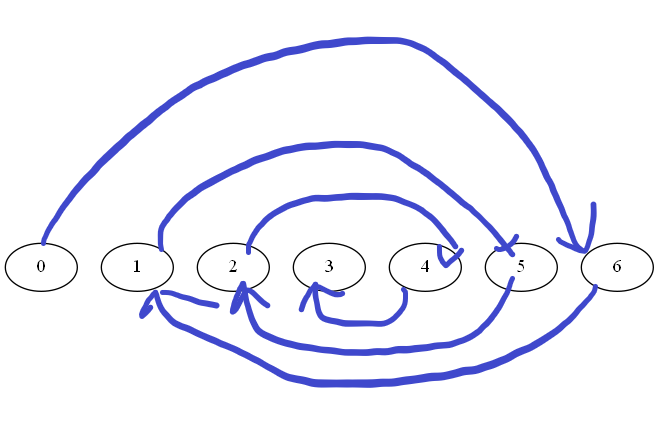
\includegraphics[width = 0.9\textwidth]{fig1.png}
        \label{fig1}
    \end{figure}

    此图遍历序列即为$6->1->5->2->4->3$, 考虑每步移动的距离,可得序列$6->(-5)->4->(-3)->2->(-1)$.

    在模6意义下即为$0->1->4->3->2->5$.

    显然如果令$a = (6,1,4,3,2,5)$,如此得到的$b$等价于每次遍历的结点编号序列,即$(6 ,1 , 5 , 2 , 4 , 3)$.

    因此我们只需构造不重的序列$a$,使得按照$a$的方式遍历刚好可以遍历每个结点恰好一次即可。

    \subsection{Solution}

    当$n$为奇数时,$b_n = \frac{n(n+1)}{2} \% n = 0.$

    因此$b_n = 1,$ 考虑$a_i = n(i\neq 1)$的情况,此时必有$b_{i} = b_{i-1}$。

    所以$b_1 = 1$.

    因此只要$n \neq 1$,$b$必有重复元素。

    当$n$为偶数时,有两种方法构造:

    \subsubsection{方法一:观察样例法}
    
    仔细观察样例(或者自己多构造几组样例),发现其形如$0,-1,2,-3,....,(-1)^{n-1} (n-1)$.

    其前缀和为$0,-1,1,-2,2,...,-\frac{n}{2}$.

    满足条件。

    \textbf{方法二:图论模型法}

    另外一种方法便是观察图论模型,可以发现$0,-(n-1),n-2,-(n-3),...,-1$也是一组解(见\ref{fig1})。

    其等价于$0,1,-2,3,...,(-1)^{n}(n-1)$.

    本质上是方法一的对称情况,证明略。

    \subsection{Code}
    
    \subsubsection{方法一}
    \lstinputlisting[language=c++]{Code_1.cpp}

    \subsubsection{方法二}
    \lstinputlisting[language=c++]{Code_2.cpp}


    \subsection{E. Making Anti-Palindromes}
    \emph{给定一个字符串$s$,定义反回文串: 如果一个字符串对于任意$i$, 都有$s[i] \neq s[n - i](i \in \{1,2,...,n\})$, 那么就称字符串$s$为反回文串。
     现在你可以进行一个交换操作, 也即交换字符串两个位置上的字符, 求最少的交换次数使得$s$变为反回文串。}

    \subsection{Solution}
    定义集合$S = \{(i,n-i) | s[i] = s[n-i] \text{且} i<n-i\}$,我们的目的便是将$S$清空。

    可以将消除分为以下两个步骤:


    \textbf{步骤1:} 观察到一个交换操作最多可以消除2个$S$中的元素$(i,n-i),(i',n-i')$,只需满足$s[i] \neq s[i']$即可。

    反复重复上述操作,最终$S$下标对应的字符将会全部相同, 记此时的集合为$S'$.
    
    \textbf{步骤2:} 对于这些字符全相同的字符,1次交换只能消除1个$S$中的元素。具体操作如下:
    
    对于$(i,n-i)$, 选择一对索引$(j,n-j)$, 其中$s[j]\neq s[i] ,s[n-j] \neq s[i]$且 $s[j]\neq s[n-j]$.

    交换$(i,j)$即可。


    现在考虑最小化操作数量,显然\textbf{步骤2}需要的操作数为$|S'|$, 因此我们需要在步骤1中最小化$|S'|$.

    记$\Count(i)$为$S$中满足$s[i] = s[i']$的索引数量,$(i,n-i),(i',n-i')\in S$。
    
    考虑$S$中任意使得$\Count$函数最大的$i$, 记为$i_{max}$.

    显然可以对于$\Count(i_{max})$进行分类讨论,

    如果$\Count(i_{max}) \geq  \sum_{\Count(i') \neq \Count(i)} \Count(i')$, 
    
    观察到此时最佳方案为每个交换$i$和$i'$,其中$\Count(i) =  \Count(i_max), \Count(i')\neq \Count(i_{max})$.

    此时$\min(|S'|) = \Count(i_{max}) -  \sum_{\Count(i') \neq \Count(i)} \Count(i')$.
    

    如果$\Count(i_{max}) < \sum_{\Count(i') \neq \Count(i)} \Count(i')$,

    

\end{document}
